\documentclass{article}
\usepackage{minted}
\input{preamble-eng}
\title{Stanford CS234: Lectures 5 to 6}
\begin{document}

\section{Lecture 5: Policy Gradient and Search}
Policy gradient/ search is influential in NLP/ Proximal Policy Optimization (training GPT). The core idea:

\begin{defbox}
    \subsubsection*{Intuition of Gradient Search}
    Approximate $V^{\pi}(s) \approx V_{W}(s)$ and $Q_w(s, a) \approx Q^{\pi}(s, a)$ by adjusting weight $w$.
    \\\textbf{Policy} gradient: rather than generating policy from value ($\epsilon$-greedy), directly parametrize policy with $\theta$, i.e.
    \begin{center}
        $\pi_{\theta} (s, a) = \mathbb{P}[a | s; \theta]$: optimize $V(\theta)$ to find policy $\pi$
    \end{center}
\end{defbox}

The brief classification of policy gradient is as follows:
\begin{center}
    \begin{tabular}{|c||c|c|c|}
    \hline
      & Value-based & Policy-based & Actor-critic \\ \hline
    Value function & learned & not present & learned \\ \hline
    Policy & implicit ($\epsilon$-greedy) & learned & learned\\ \hline
    \end{tabular}
\end{center}

Instead of deterministic/ $\epsilon$-greedy policies, need to focus heavily on \textbf{stochastic} for direct policy search!
\begin{itemize}
\item Repeated Trials, e.g. In rock paper scissors (of many rounds), deterministic policy is easily exploited by adversary.
\item Boundary Condition, e.g. In gridworld, bound to only move one direction (else get stuck/ traverse for long time for slow convergence).
\end{itemize}

In short, poliy objective functions have the following intuition:
\begin{defbox}
    \subsubsection*{Policy Objective Summary}
    \begin{itemize}
    \item Goal: Given policy $\pi_{\theta}(s, a)$, find best parameter $\theta$.
        \\Inherently, an optimization of $V(s_0, \theta)$.
    \item Purpose: Measure quality for policy $\pi_{\theta}$ with policy value at start state $s_0$.
    \item Works for: both episodic/ continuing and infinite horizons.
    \end{itemize}
\end{defbox}

\subsection{Gradient Free Policy Optimization}
They are great simple baselines.
\begin{itemize}
\item Examples: Hill Climbing, Genetic Algo (evolution strategies, cross-entropy method, covariance matrix adaption)
\item Known for decades but embarrassingly well: rivals standard RL techniques!
\item Advantages: Flexible for any policy parameterization, easily to parallelize
    \\Disadvantage: Less sample efficient (ignores temporal structure)
\end{itemize}

\subsection{Policy Gradient}
This section focuses on gradient descent; other popular algos include conjugate gradient and quasi-newton methods.
\\Usually assume \textbf{Episodic MDPs} for easy extension of objectives. The method:
\begin{thmbox}
    Define $V(\theta) = V(s_0, \theta)$, i.e. the value fucntion depending on policy parameters. Then:
    \begin{itemize}
    \item Search the local maximum in $V(s_0, \theta)$ with gradient increments:
        \begin{equation*}
            \Delta \theta = \alpha \nabla_{\theta} V(s_0, \theta) = \alpha
            \begin{pmatrix}
                \frac{\partial V(s_0, \theta)}{\partial \theta_{1}} \\
                \vdots \\
                \frac{\partial V(s_0, \theta)}{\partial \theta_{n}}
            \end{pmatrix}
        \end{equation*}
    \item Assumption: $\pi_{\theta}$ differentiable (and known gradient $\nabla_{\theta} \pi_{\theta}(s, a)$)
    \item We can rewrite policy value $V(s_0, \theta)$ in the following ways:
        \begin{enumerate}
        \item \textbf{Visited States and Actions}: 
            $\mathbb{E}_{\pi_{\theta}} \left[ \sum_{t = 0}^{T} R(s_t, a_t); \pi_{\theta}, s_0 \right]$
        \item \textbf{Weighted Average of Q-values by Actions}:
            $\sum_{a} \pi_{\theta} (a | s_0) Q(s_0, a, \theta)$
        \item \textbf{Trajectories Sampled using $\pi_{\theta}$}: 
            $\sum_{\tau} P(\tau | \theta) R(\tau)$
        \end{enumerate}
    \end{itemize}
\end{thmbox}

In particular, it is of interest to consider writing $V(s_0, \theta)$ in trajectory form:
\begin{prfbox}
    To find the best policy parameter $\theta$, we consider
    \begin{equation*}
        \mathop{\arg\max}\limits_{\theta} V(\theta)
        =
        \mathop{\arg\max}\limits_{\theta} \sum_{\tau} P(\tau ; \theta) R(\tau)
    \end{equation*}
    Taking gradient,
    $\begin{aligned}
        \nabla_{\theta} V(\theta) =
        & \nabla_{\theta} \sum_{\tau} P(\tau; \theta) R(\tau) \\
        & \sum_{\tau} \nabla_{\theta} P(\tau; \theta) R(\tau) \text{($R$ being indep of $\theta$)}\\
        & \sum_{\tau} \frac{P(\tau; \theta)}{P(\tau; \theta)} \nabla_{\theta} P(\tau; \theta) R(\tau) \\
        & \sum_{\tau} R(\tau) P(\tau; \theta) \nabla_{\theta} \textcolor{orange}{\log P(\tau; \theta)} ~~~~\text{(log-likelihood)} \\
    \end{aligned}$

    \textbf{Approximate} in practice using $m$ sample trajectories under $\pi_{\theta}$:
    \begin{equation*}
        \nabla_{\theta} V(\theta) \approx \hat{g} = \frac{1}{m} \sum_{i = 1}^{m} R(\tau^{(i)}) \nabla_{\theta} \log P(\tau^{(i)}, \theta)
    \end{equation*}
\end{prfbox}

But trajectories can be decomposed into states and actions:
\begin{prfbox}
    $\begin{aligned}
        \nabla_{\theta} \log P(\tau^{(i)}; \theta) =
        & \nabla_{\theta} \log \left[ \textcolor{cyan}{\mu(s_0)} 
            \textcolor{magenta}{\prod_{t = 0}^{T-1} \pi_{\theta} (a_t | s_t)}
            \textcolor{orange}{P(s_{t+1} | a_{t+1}, s_{0:t}, a_{0:t})} \right] \\
        & =\textcolor{magenta}{\sum_{\tau}} \nabla_{\theta} \log \textcolor{magenta}{\pi_{\theta} (a_t | s_t)} \\
    \end{aligned}$
\end{prfbox}

Here 
    \begin{itemize}
    \item We call $\sum_{\tau} \nabla_{\theta} \log \pi_{\theta} (a_t | s_t)$ the \textbf{score function}.
    \item \textcolor{cyan}{the initial state $\mu(s_0)$ is constant};  
        \textcolor{orange}{dynamics model $P(s_{t+1} | a_{t+1}, s_{0:t}, a_{0:t})$ is invariant to $\theta$.}
    \item In other words, no dynamics model is required to approximate the policy parameter $\theta$.
    \end{itemize}

\begin{hintbox}
    \textbf{Questions}
    \begin{enumerate}
    \item Why trajectory form is practical ("better in training")?
    \item Why is log-likelihood ratio important here? What does it enable?
    \end{enumerate}
\end{hintbox}

\subsection{Selecting a Right Policy}

\subsubsection{Softmax Policy}
\begin{itemize}
\item In softmax, \textbf{exponentially weight} quantities of linear combination of features as probabilities (that add to 1):
    \begin{equation*}
        \pi_{\theta}(s, a) = \frac{e^{\phi (s, a)^{T} \theta}}{\sum_{a} e^{\phi (s, a)^{T} \theta}}
    \end{equation*}
\item Then the score function can be written as 
    $\nabla_{\theta}(s, a) = \phi(s, a) - \mathbb{E}_{\pi_{\theta} [ \phi(s, \cdot) ]}$
\end{itemize}

\subsubsection{Gaussian Policy}
\begin{itemize}
\item A normal distribution is natural for continuous action spaces; at times used by deep NN.
\item Action $a \sim N(\mu(s), \sigma^2)$. Mean $\mu(s) = \textcolor{cyan}{\phi(s)}^{T} \textcolor{orange}{\theta}$ is a \textcolor{orange}{linear combination} of \textcolor{cyan}{state features}. 
\item Then the score function can be written as $\nabla_{\theta}(s, a) = \phi(s, a) - \mathbb{E}_{\pi_{\theta}} \left[ \phi(s, \cdot)\right]$
\end{itemize}

When to use policy gradient?
\begin{enumerate}
\item Differentiable reward functions
\item No dynamics required
\item Useful for both infinite horizon and episodic settings
\item Intuition: $R(\tau^{(i)})$ is replacable by other functions that \textit{measures the wellness of sample $x$}
    \\Essentially, moving in the direction of $\hat{g_{i}} = f(x_i) \nabla_{\theta} \textcolor{orange}{\log p(x_i | \theta)}$ pushes up the \textcolor{orange}{log probability} proportionally.
\end{enumerate}

\begin{hintbox}
    What are the purposes of selecting Softmax and Gaussian policies?
\end{hintbox}

The generalization is as follows:
\begin{thmbox}
    \subsubsection*{Policy Gradient Theorem}
    Assumption: Differentiable Policy $\pi_{\theta}(s, a)$, objective $J = 
    \begin{aligned}
        J_1 & \text{(Episodic)} \\
        J_{avR} & \text{(Avg. Reward over time)} \\
        \frac{1}{1 - \gamma} J_{avV} & \text{(Avg. Value over time)} \\
    \end{aligned}$
    
    In any case, the policy gradient is 
    $\nabla_{\theta} J(\theta) = \mathbb{E}_{\pi_{\theta}} \left[ \nabla_{\theta} \log \pi_{\theta} (s, a) Q^{\pi_{\theta}} (s, a)\right]$
\end{thmbox}

\subsubsection*{Summary and Improvements of Policy-based RL}
\begin{center}
    \begin{tabular}{|c||c|c|}
    \hline
    Criteria & Advantages & Disadvantages \\ \hline
    Convergence & Better Properties & Typical Local Optimum \\ \hline
    Flexibility & Effective in high-dim./ continuous action spaces & Inefficient, high-variance \\ 
    & Can learn stochastic policies & policy evaluation \\ \hline
    \end{tabular}
\end{center}

\begin{defbox}
    Currently, use
    \begin{equation*}
        \nabla_{\theta} V(\theta) = \frac{1}{m} \sum_{i = 1}^{m} R(\tau^{(i)}) \sum_{t = 0}^{T-1} \nabla_{\theta} \log \pi_{\theta} (a_t^{(i)}, s_t^{(i)})
    \end{equation*}
    to estimate
    \begin{equation*}
        \nabla_{\theta} \mathbb{E}_{\tau} [R] = \mathbb{E}_{\tau} \left[ \left(\sum_{t = 0}^{T-1} r_{t} \right) \sum_{t=0}^{T-1} \nabla_{\theta} \log \pi_{\theta} (a_t | s_t) \right]
    \end{equation*}
    It is unbiased but \textcolor{red}{noisy (high variance)!}
\end{defbox}
On the high variance, several remedies serve as improvements:

\subsubsection{Fix 1: Temporal Structure}
\begin{itemize}
\item Focus on \textcolor{blue}{single reward item} at once:
    \begin{equation*}
        \nabla_{\theta} \mathbb{E}[\textcolor{blue}{r_{t'}}] = \mathbb{E}[r_{t'} \sum_{t = 0}^{t'} \nabla_{\theta} \log \pi_{\theta} (a_t | s_t)]
    \end{equation*}
\item \textcolor{orange}{Sum up over $t$} to obtain:
    $\begin{aligned}
        V(\theta) = \nabla_{\theta} \mathbb{E}[\textcolor{orange}{R}] & 
        = \mathbb{E} [ \textcolor{orange}{\sum_{t' = 0}^{T-1} r_{t'}} \sum_{t = 0}^{t'} \nabla_{\theta} \log \pi_{\theta} (a_t | s_t)] \\
        & = \mathbb{E} [ \sum_{t = 0}^{T-1} \nabla_{\theta} \log \pi_{\theta} (a_t , s_t) \textcolor{orange}{\sum_{t' = t}^{T-1} r_{t'}}] \quad \text{(because later decisions don't influence past rewards)}\\
    \end{aligned}$
\item This can be further simplified: trajectory $\tau^{(i)}$ has return \textcolor{orange}{$G_t^{(i)} = \sum_{t' = t}^{T-1} r_{t'}^{(i)}$}. Hence
    \begin{equation*}
        \nabla_{\theta} \mathbb{E}[R] \approx \frac{1}{m} \sum_{i = 1}^{m} \sum_{t = 0}^{T-1} \nabla_{\theta} \log \pi_{\theta} (a_t, s_t) \textcolor{orange}{G_t^{(i)}}
    \end{equation*}
\end{itemize}

\begin{thmbox}
    \subsubsection*{Monte-Carlo Policy Gradient}
    Making use of likelihood ratio / score function and temporal structure, update param $\theta$ with
    \begin{equation*}
        \Delta \theta_{t} = \alpha \nabla_{\theta} \log \pi_{\theta} (s_t, a_t) G_{t}
    \end{equation*}
    after initializing $\theta$ arbitrarily.
\end{thmbox}

\begin{hintbox}
    Q: How does Temporal structure reduce variance?
\end{hintbox}

\subsubsection{Fix 2: Baseline Function}
As iteration costs time and computational resources, we desire \textcolor{blue}{quick convergence} to local optima.

\begin{thmbox}
    \subsubsection*{Baselines: Unbiasedness and Other Considerations}
    $\nabla_{\theta} \mathbb{E}_{\tau} [R] = \mathbb{E}_{\tau} \left[ \left(\sum_{t' = t}^{T-1} r_{t'} \textcolor{magenta}{- b(s_t)} \right) \sum_{t=0}^{T-1} \nabla_{\theta} \log \pi_{\theta} (a_t | s_t) \right]$

    \textbf{Why it works?}
    \begin{itemize}
    \item Unbiased for any $b$ if $b$ is a function of $s$ but not $\theta$, because
        \\$\mathbb{E}_{\tau} \left[ \nabla_{\theta} \log \pi(a_t | s_t; \theta) b(s_t) \right] = 0$
    \item A near-optimal baseline choice is the expected return 
        $b(s_t) \approx \mathbb{E} \left[ \sum_{t' = t}^{T-1} r_{t'} \right]$
    \item Other choices: State-value function $V^{\pi}(s) = \mathbb{E}_{a \sim \pi} \left[ Q^{\pi} (s, a) \right]$
    \end{itemize}
    \textbf{Interpretation}: Increase logprob of action at proportionally to how much returns 
    $\sum^{T-1}_{t'= t} r_{t'}$ are better than expected
\end{thmbox}

\begin{hintbox}
    Q: Intuitively, what are the uses of baseline functions? How does variance get reduced?
    \begin{prfbox}
        \textbf{Core idea: Break down $t$} in the summation:
        \begin{itemize}
        \item As we sample from trajectories $\tau$ (MC),
            $\begin{aligned}
                \text{Var}[ \nabla_{\theta} [R]] & 
                = \text{Var}[ \sum_{t = 0}^{T-1} \nabla_{\theta} \log \pi(a_t | s_t; \theta) (R_t (s_t) - b(s_t))]\\ & 
                \approx \sum_{t = 0}^{T-1} \mathbb{E}_{\tau} \left[ \text{Var}[\nabla_{\theta} \log \pi(a_t|s_t ; \theta) (R_t(s_t) - b(s_t))] \right]\\
            \end{aligned}$
        \item For each $t$, write variance Var$[X]$ as $\mathbb{E}[X^2] - (\mathbb{E}[X])^2$:
            \\$\mathbb{E}\left[\left((\nabla_{\theta} \log \pi(a_t | s_t ; \theta)) (R_t(s_t) - b(s_t)) \right)^2 \right]
            - \mathbb{E}\left[\left((\nabla_{\theta} \log \pi(a_t | s_t ; \theta)) (R_t(s_t) - b(s_t)) \right) \right]^2$
        \item Second term is not affected by choice of $b(s)$ (unbiased = same expectation). The variance equals
            $\mathop{\arg\min}\limits_{b} ~~\mathbb{E}\left[\left((\nabla_{\theta} \log \pi(a_t | s_t ; \theta))\right)^2 \left((G_t(s_t) - b(s_t)) \right)^2 \right]$
            \\$=\mathop{\arg\min}\limits_{b} ~~\mathbb{E}_{s \sim d^{\pi}}\left[ \mathbb{E}_{a \sim \pi(\cdot | s), G | s, a} \left[ \left((\nabla_{\theta} \log \pi(a_t | s ; \theta))\right)^2 \left((G_t(s_t) - b(s_t)) \right)^2 \right] \right]$
        \item A \textbf{weighted least-squares} problem that minimizes
            \begin{equation*}
                \sum_{i} \sum_{t} |b(s^{i}_{t}) - \textcolor{blue}{G^{i}_{t}}|^2 \quad\quad \text{(\textcolor{blue}{$G$ (or $A = G - b$)} being target)}
            \end{equation*}            
            with solution (after taking zero gradient)
            \begin{equation*}
                b(s) \approx \mathbb{E}_{a \sim \pi(\cdot | s), G | s, a} [G_t (s)]
            \end{equation*}
        \end{itemize}
    \end{prfbox}

    Q: What does it mean by "Near optimal"? When is it not?
\end{hintbox}

\subsubsection{Fix 3: Alternative to MC}
The original $G_{t}^{i}$ estimates expected discounted sum of returns (from single roll): unbiased but \textcolor{red}{high variance}.
To solve this:
\begin{itemize}
\item Leverage \textcolor{cyan}{bootstrapping and approximation} (similar to TD vs MC and VFA) to introduce bias.
\item Use "Critic" to estimate the ratio $\frac{V}{Q}$. The popular class of "Actor-critic" methods explicitly represents (and updates) policy and values.
\item Essentially, replace $\sum_{t' = t}^{T-1} r_{t'} - b(s_t)$ \textcolor{orange}{[Vanilla MC]} 
    with Q-values ($Q(s_t, a_t; \mathbf{w}) - b(s_t)$) \textcolor{orange}{[This is essentially TD]} 
    \\or advantage function $\hat{A}^{\pi}(s_t, a_t)$ where $A^{\pi}(s, a) = Q^{\pi}(s, a) - V^{\pi}(s)$.
\end{itemize}

\begin{thmbox}
    \subsubsection*{Alternative Targets to MC Estimators}
    With vanilla MC, the gradient is estimated by
    \begin{equation*}
        \nabla_{\theta} V(\theta) \approx \frac{1}{m} \sum_{i = 1}^{m} \sum_{t = 0}^{T-1} \textcolor{blue}{R_{t}^{i}} \nabla_{\theta} \log \pi_{\theta} (a_t^{(i)} | s_t^{(i)})
    \end{equation*}

    \textbf{Proposed replacements:}
    \begin{enumerate}
    \item N-step estimators:
        \begin{itemize}
        \item $\hat{R}_t^{(1)} = r_t + \gamma V(s_{t+1})$, $\hat{R}_t^{(2)} = r_t + \gamma r_{t+1} + \gamma^2 V(s_{t+2})$ 
        \item $\hat{R}_t^{(\infty)} = r_t + \gamma r_{t+1} + \gamma r_{t+2} + \dots$
        \end{itemize}
    \item Advantage estimators, by \textit{\textcolor{orange}{subtracting baselines of $V(s_t)$} from above}
        \begin{itemize}
        \item $\hat{A}_t^{(1)} = \hat{R}_t^{(1)} \textcolor{orange}{- V(s_t)} = r_t + \gamma V(s_{t+1}) \textcolor{orange}{- V(s_t)}$ \quad \quad 
            \quad \quad \textcolor{blue}{(\textit{low variance, high bias})}
        \item $\hat{R}_t^{(\infty)} \textcolor{orange}{- V(s_t)} = r_t + \gamma r_{t+1} + \gamma r_{t+2} + \dots \textcolor{orange}{- V(s_t)}$
            \quad \quad \textcolor{blue}{(\textit{high variance, low bias})}
        \end{itemize}
    \end{enumerate}
\end{thmbox}

\begin{hintbox}
    What does the word "critic" here mean?
\end{hintbox}

A summary of policy gradient:

\begin{defbox}
    \subsubsection*{Intermediate Summary of PG}
    \begin{itemize}
    \item Core idea: $\nabla_{\theta} V(\theta) = \mathbb{E}_{\pi_{\theta}} \left[ \nabla_{\theta} \textcolor{cyan}{\log \pi_{\theta} (s, a)} \textcolor{blue}{Q^{\pi_{\theta}} (s, a)} \right]$
        \\\begin{prfbox}
            Optimize $\mathop{\arg\max}\limits_{\theta} J(\pi_{\theta}) = \mathbb{E}_{\tau \sim \pi_{\theta}} \left[ \sum_{t = 0}^{\infty} \gamma^{t} r_{t}\right]$ with SGD on $\theta$:
            \begin{equation*}
                g = \nabla_{\theta} J(\pi_{\theta}) = \mathbb{E}_{\tau \sim \pi_{\theta}} \left[ \sum_{t = 0}^{\infty} \gamma^{t} \nabla_{\theta} \log \pi_{\theta} (a_t | s_t) A^{\pi_{\theta}} (s_t, a_t) \right]
            \end{equation*}
        \end{prfbox}
    \item State-action pairs with higher $\hat{Q}$ increases probabilities in average
    \item Direction of $\theta$ dependent on gradient of \textcolor{cyan}{$\ln \pi(S_t, A_t, \theta)$} AND \textcolor{blue}{Q-values/ returns}
    \item NOT guaranteed to converge to global optima (just local!)
    \end{itemize}
\end{defbox}

\subsection{Limitations of Vanilla Policy Gradient}
    A PG algo should minimize \# iterations to reach a good (probably suboptimal) policy within time. The limitations of vanilla PG:
    \subsubsection{Poor sample efficiency}
    Variance reduces slowly, because PG is an \textbf{on-policy} expectation: Data immediately \textcolor{red}{discarded} after just one gradient step
    \begin{itemize}
    \item Collect sample estimates from trajectories of same policy (more stable), or \textcolor{magenta}{other policies (off-policy, less stable)}.
    \item Opportunity: Can we take \textcolor{blue}{multiple gradient steps from old data} before new policy?
    \end{itemize}

    \begin{defbox}
        \subsubsection*{Problems of Determining Gradient Step}
        Problem: Difficult to handle step size (dist. in parameter space $\neq$ dist. in policy space)
        \begin{itemize}
        \item e.g. Matrices in tabular case $\Pi = \{ \pi: \pi \in \mathbb{R}^{|S| \times |A|}, \sum_{a} \pi_{s_a} = 1, \pi_{s_a} \geq 0 \}$
            \\VS steps of policy gradient in parameter space $\implies$ \textcolor{magenta}{unable to map/ gauge size}!
        \item SGD of $\theta_{k+1} = \theta_{k} + \alpha_{k} \hat{g}_k$ is subject to \textcolor{red}{performance collapse} with large steps!
            \\e.g. logistic function: small $\Delta \theta$ leads to big policy changes
        \end{itemize}
    \end{defbox}

    The solution to restrict policy change from more than intended is through \textcolor{blue}{policy performance bounds}:
    \begin{defbox}
        \subsubsection*{Distance in Value to Policy}
        To respect distance mapping in policy space, exploit relationships between policy performance:
        \begin{equation*}
            J(\pi') - J(\pi) = \mathbb{E}_{\tau \sim \pi'} \left[ \sum_{t = 0}^{\infty} \gamma^{t} A^{\pi}(s_t, a_t) \right]
            = \frac{1}{1-\gamma} \mathbb{E}_{s \sim d^{\pi'}, a \sim \pi'} \left[ A^{\pi} (s, a) \right]
        \end{equation*}
        Here $d^{\pi}(s) = (1 - \gamma) \sum_{t = 0}^{\infty} \gamma^{t} P(s_t = s | \pi)$ is the \textbf{weighted} distribution of states. Making use,

        Now, rewrite the objective:
        $\begin{aligned}
            \mathop{\max}\limits_{\pi'} J(\pi') & = \mathop{\max}\limits_{\pi'} J(\pi') - J(\pi) & = \mathop{\max}\limits_{\pi'} \mathbb{E}_{\tau \sim \pi'} \left[ \sum_{t = 0}^{\infty} \gamma^{t} A^{\pi}(s_t, a_t) \right] \\
            & & = \mathop{\max}\limits_{\pi'} \frac{1}{1-\gamma} \mathbb{E}_{s \sim d^{\pi'}, a \sim \pi'} \left[ A^{\pi} (s, a) \right] \\ 
            & & = \mathop{\max}\limits_{\pi'} \frac{1}{1-\gamma} \mathbb{E}_{s \sim d^{\pi'}, \textcolor{red}{a \sim \pi}} \left[ \textcolor{red}{\frac{\pi' (a | s)}{\pi(a | s)}} A^{\pi} (s, a) \right]
        \end{aligned}$
    \end{defbox}

    \textbf{Why rewrite?}
    \begin{enumerate}
    \item Now, performance of $\pi'$ is defined in advantages from $\pi$.
    \item Requires trajectories sampled from $\pi'$ (desired: from $\pi$ because our tweak features \textcolor{red}{$s \sim d^{\pi}$}).
    \end{enumerate}

    We have a useful approximation:
    \begin{thmbox}
        \subsubsection*{Relative Policy Performance Bounds}
        \begin{equation*}
            J(\pi') - J(\pi) \approx \mathbb{L}_{\pi} (\pi') \quad\quad \text{for close $\pi'$ and $\pi$ ($d^{\pi'} = d^{\pi}$)}
        \end{equation*}
        Approximation quality is ensured by relative policy performance bounds:
        \begin{equation*}
            |J(\pi') - \left( J(\pi) + \mathbb{L}_{\pi} (\pi') \right)| \leq C \sqrt{\mathbb{E}_{s \sim d^{\pi}} \left[ D_{KL} (\pi' || \pi) [s]\right]}
        \end{equation*}
    \end{thmbox}
    
    But what is $\mathbb{E}_{s \sim d^{\pi}} \left[ D_{KL} (\pi' || \pi) [s]\right]$? 
    \begin{defbox}
        \subsubsection*{KL-Divergence}
        Such divergence measures distance between \textcolor{blue}{probability distributions}:
        \begin{equation*}
            D_{KL} (P || Q) = \sum_{x} P(x) \log \frac{P(x)}{Q(x)}
        \end{equation*}
        KL satisfies $D_{KL}(P || P) = 0, D_{KL}(P || Q) \geq 0, D_{KL}(P || Q) \neq D_{KL}(Q || P)$.

        Between policies, $D_{KL}(\pi' || \pi) [s] = \sum_{a \in A} \pi' (a | s) \log \frac{\pi' (a | s)}{\pi (a | s)}$
    \end{defbox}

    After the approximation, we can optimize using trajectories \textcolor{blue}{sampled from the old policy $\pi$}!
    \begin{thmbox}
        \subsubsection*{Policy Optimization under Bounded KL Approximation}
        Policy improvement can be estimated by sampling from \textcolor{red}{old policy $\pi$}!
        \begin{equation*}
            J(\pi') - J(\pi) \approx L_{\pi}(\pi') 
            = \mathbb{E}_{\textcolor{red}{\tau \sim \pi}} \left[ \sum_{t = 0}^{\infty} \gamma^{t} \frac{\pi'(a_t, s_t)}{\pi(a_t, s_t)} A^{\pi}(s_t, a_t) \right]
        \end{equation*}
    \end{thmbox}

\subsection{Proximal Policy Optimization (PPO): Approximation in Action}
PPO penalizes large policy change iterations. There are two methods: 
\begin{enumerate}
\item regularization term on KL-divergence (Adaptive Penalty)
\item pessimistic objective on far-away policies (Clipped Objective)
\end{enumerate}

\begin{thmbox}
    \subsubsection*{PPO Iterative Algorithm - Adaptive Penalty}
    \begin{equation*}
        \theta_{k+1} = \mathop{\arg\max}\limits_{\theta} L_{\theta_k} (\theta) - \beta \bar{D}_{KL} (\theta || \theta_k)
    \end{equation*}
    Here, KL-divergence is an expectation:
    \begin{equation*}
        \bar{D}_{KL} (\theta || \theta_k) = \mathbb{E}_{s \ sim d^{\pi_k}} D_{KL} \left( \theta_{k} (\cdot | s), \pi_{\theta} (\cdot | s) \right)
    \end{equation*}
    Penalty coefficient $\beta_k$ changes between iterations:
    \begin{itemize}
    \item Initiate policy param $\theta_0$, initial KL penalty $\beta_0$, target KL-divergence $\delta$
    \item Compute policy update (iterate $\theta$) by K steps of minibatch SGD (via Adam)
    \item Control KL-divergence to be around $\delta$ by adjusting penalty:
        \\If $\bar{D}_{KL} (\theta || \theta_k) \geq 1.5 \delta$ then $\beta_{k+1} = 2 \beta_{k}$;
        \\elif $\bar{D}_{KL} (\theta || \theta_k) \leq \frac{\delta}{1.5}$ then $\beta_{k+1} = \frac{1}{2} \beta_{k}$
    \end{itemize}
    This KL penalty is called "adaptive" because of \textcolor{orange}{how $\beta_k$ changes (adapts quickly)} according to KL-divergence.
\end{thmbox}

An alternative approach is clipping: restrict via \textcolor{blue}{pessimistically treating objective value far away from $\theta_k$}.
\begin{thmbox}
    \subsubsection*{Outline of Clipped Objective on Policy Changes}
    \begin{itemize}
    \item Define relative probability change: $r_{t}(\theta) = \frac{\pi_{\theta} (a_t | s_t)}{\pi_{\theta_k} (a_t | s_t)}$ 
    \item The new objective is
        \begin{equation*}
            L_{\theta_{k}}^{\text{Clip}} (\theta) 
            = \mathbb{E}_{\tau \sim \pi_{k}} \left[ \sum_{t = 0}^{T} \left[ \textcolor{magenta}{\min} \left( r_{t} (\theta) \hat{A}_t^{\pi_{k}}, \textcolor{blue}{\text{clip}(r_{t}(\theta), \textcolor{orange}{1 - \epsilon, 1 + \epsilon})} \hat{A}_t^{\pi_{k}} \right) \right] \right]
        \end{equation*}
        In other words, $r_{t} (\theta)$ is \textcolor{blue}{clipped between ($\textcolor{orange}{1 - \epsilon, 1 + \epsilon}$)}; hyperparameter $\epsilon$ usually set at 0.2.
    \item Policy update: $\theta_{k+1} = \mathop{\arg\max} ~~~ \limits_{\theta} L_{\theta_{k}}^{\text{Clip}} (\theta)$
    \end{itemize}
\end{thmbox}

Here, Clipping discentivizes going far from $\theta_{k+1}$:
\begin{itemize}
\item Left graph below: when the advantage function $A > 0$; right graph when $A < 0$.
\item $L_{\theta_{k}}^{\text{Clip}} (\theta)$'s increase is suppressed at extreme values towards the sign of $A$.
\item Clipping is simple to implement but works well compared to KL penalty.
\end{itemize}

\begin{figure}
    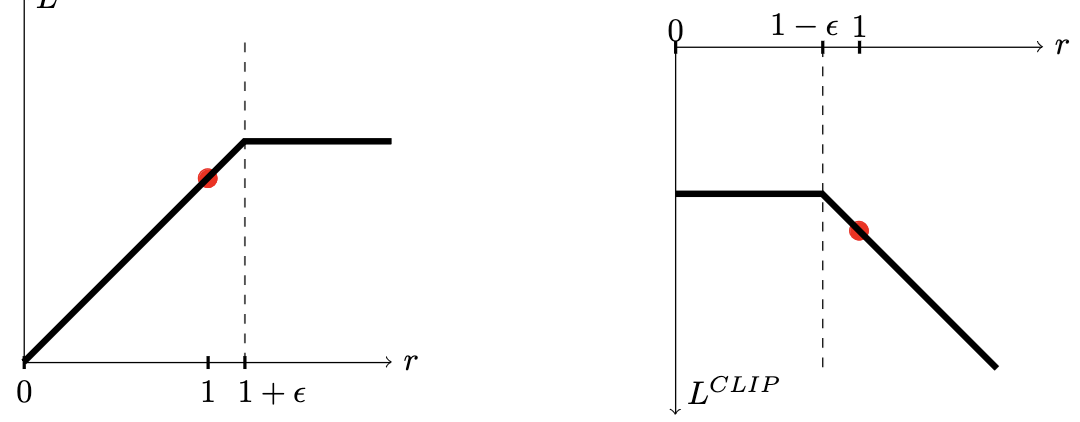
\includegraphics[width=0.8\textwidth]{lec6-clipped-values.png}
\end{figure}

PPO's performance consistently \textcolor{blue}{tops other algos, hence wildly popular.}
\begin{itemize}
\item Today, it is a key component of ChatGPT (readings: \href{https://openai.com/index/openai-baselines-ppo/}{OpenAI blog (2017)}, \href{https://arxiv.org/pdf/1707.06347}{Publication by Schulman et. al. (2017)})
\item Different outcomes with reward scaling/ learning rate annealing.
\end{itemize}



\begin{hintbox}
    Q1: Why KL-divergence applied is an expectation?
    Q2: How does the two methods compare?
\end{hintbox}

\end{document}